%% Based on a TeXnicCenter-Template by Gyorgy SZEIDL.
%%%%%%%%%%%%%%%%%%%%%%%%%%%%%%%%%%%%%%%%%%%%%%%%%%%%%%%%%%%%%

%------------------------------------------------------------
%
\documentclass[landscape, notitlepage]{article}%
%Options -- Point size:  10pt (default), 11pt, 12pt
%        -- Paper size:  letterpaper (default), a4paper, a5paper, b5paper
%                        legalpaper, executivepaper
%        -- Orientation  (portrait is the default)
%                        landscape
%        -- Print size:  oneside (default), twoside
%        -- Quality      final(default), draft
%        -- Title page   notitlepage, titlepage(default)
%        -- Columns      onecolumn(default), twocolumn
%        -- Equation numbering (equation numbers on the right is the default)
%                        leqno
%        -- Displayed equations (centered is the default)
%                        fleqn (equations start at the same distance from the right side)
%        -- Open bibliography style (closed is the default)
%                        openbib
% For instance the command
%           \documentclass[a4paper,12pt,leqno]{article}
% ensures that the paper size is a4, the fonts are typeset at the size 12p
% and the equation numbers are on the left side
%
\usepackage{graphicx}
\usepackage{tikz}
\usetikzlibrary{shapes.symbols, 
		arrows,
		decorations.pathmorphing,
		positioning,
		backgrounds,
		fit}
%-------------------------------------------

\begin{document}
\pagenumbering{gobble}
\topmargin=-10pt
\footskip=0pt
\center\small{SQW Component Interaction: \large{Initial Display upon Login}}

\begin{tikzpicture}[place/.style={
					circle,
					draw=blue!50,fill=blue!20,thick,
					inner sep=0pt,minimum size=6mm},
			component/.style={
					rectangle,
					draw=black!50,fill=blue!20,thick,
					inner sep=10pt,minimum size=10mm},
			every label/.style=red,
			bend angle=40,
			pre/.style={<-,shorten <=1pt,>=stealth',semithick},
			post/.style={->,shorten >=1pt,>=stealth',semithick}]
%% -------------- GRID ----------------------------------------- %%
	\path[help lines, blue!20, draw] grid (12,12);

%%  -------------- STICK USER 1 ------------------------------ %%
	\node [xshift=70pt, yshift=-25pt] (user1) at (2, 12)
		{ 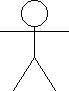
\includegraphics[width=0.6cm]{../img/stick.png}};
	\node [xshift=35pt, left=of user1] {Users};
	\node [below right=of user1,xshift=-70pt, yshift=15pt] (desktop)
		{ 
\includegraphics[width=0.8cm]{../img/desktop.jpg}}	
		edge[pre, bend left] (user1);
		
%%  -------------- STICK USER 2 ------------------------------ %%
	\node [right=of user1, xshift=2cm, yshift=-6pt] (user2)
		{ 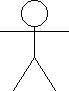
\includegraphics[width=0.6cm]{../img/stick.png}}; 
	\node [below right=of user2, xshift=-25pt, yshift=20pt] (mobile)
				{ 
\includegraphics[width=0.8cm]{../img/mobile.jpg}}
		edge[pre, bend right] (user2);	 


%% -------------- WEB SITE COMPONENT --------------------- %%
	\node [ component,below left=of desktop, xshift=1.3cm,yshift=15pt] {SqrWalla Web Site};

%% ------------------------------ GATEWAY----------------------- %%
	\node [ component,below right=of desktop, xshift=1.3cm,yshift=15pt,minimum size=30mm] {SqrWalla Gateway};

\end{tikzpicture}


\end{document}
